\documentclass[slideColor,colorBG,nototal,blends,pdf]{prosper}

\usepackage{color}
\usepackage{epsfig}

\newcommand{\jbPerf}{\textsf{\normalsize jbPerf}}
\newcommand{\enzo}{\textsf{\normalsize Enzo}}
\newcommand{\hypre}{\textsf{\textit{\normalsize hypre}}}
\newcommand{\code}[1]{\textsf{\small #1}}
\newcommand{\indvar}{r}
 \newcommand{\uc}{u(\indvar)}
 \newcommand{\ac}{a(\indvar)}


\definecolor{titlecol}{rgb}{0,0,0.5}

\title{\textcolor{titlecol}{\textit{AMR RT}}}

\author{\textcolor{blue}{James Bordner}}
\email{\textcolor{blue}{jobordner@ucsd.edu} \\
        \textcolor{blue}{2007-04-18}}
\institution{\textcolor{red}  {Laboratory for Computational Astrophysics} \\
             \textcolor{red}{Center for Astrophysics and Space Sciences} \\
             \textcolor{red}{University of California, San Diego}}

 \DefaultTransition{Replace}

%======================================================================
\begin{document}

\raggedright

%\maketitle

%=======================================================================
\begin{slide}{\large AMR RT Plan}
\small
\begin{itemize}
\item AMR effort is largely orthogonal to unigrid effort
\item Just getting underway
\item Three main steps:
\begin{enumerate}
\item discretize and solve linear problems on composite AMR grids via \hypre's \code{SStruct} interface
\item incorporate the linear solver into \enzo's hierarchical time-stepping scheme
\item develop and run AMR RT test problems
\end{enumerate}
\end{itemize}
\end{slide}
%=======================================================================
\begin{slide}{\large AMR RT Plan: Step 1\\
              \normalsize  linear solution}
\small
\begin{itemize}
\item Currently writing a test program for experimenting with AMR discretizations and \hypre\ solvers
\begin{itemize}
\item Problem: $\nabla\cdot(a \nabla u) = f$
 \item pass 1:
\begin{itemize}
\item $a\equiv 1$: self-gravity
\item refinement factor $r=2$
\item $f$ based on point/spherical masses
 \end{itemize}
\end{itemize}
\item Code will be reused when interfacing with \enzo
\end{itemize}
\end{slide}

%=======================================================================
\begin{slide}{\large AMR RT Plan: Step 1a\\
              \normalsize  discretization}
\small
\begin{minipage}{1.75in}
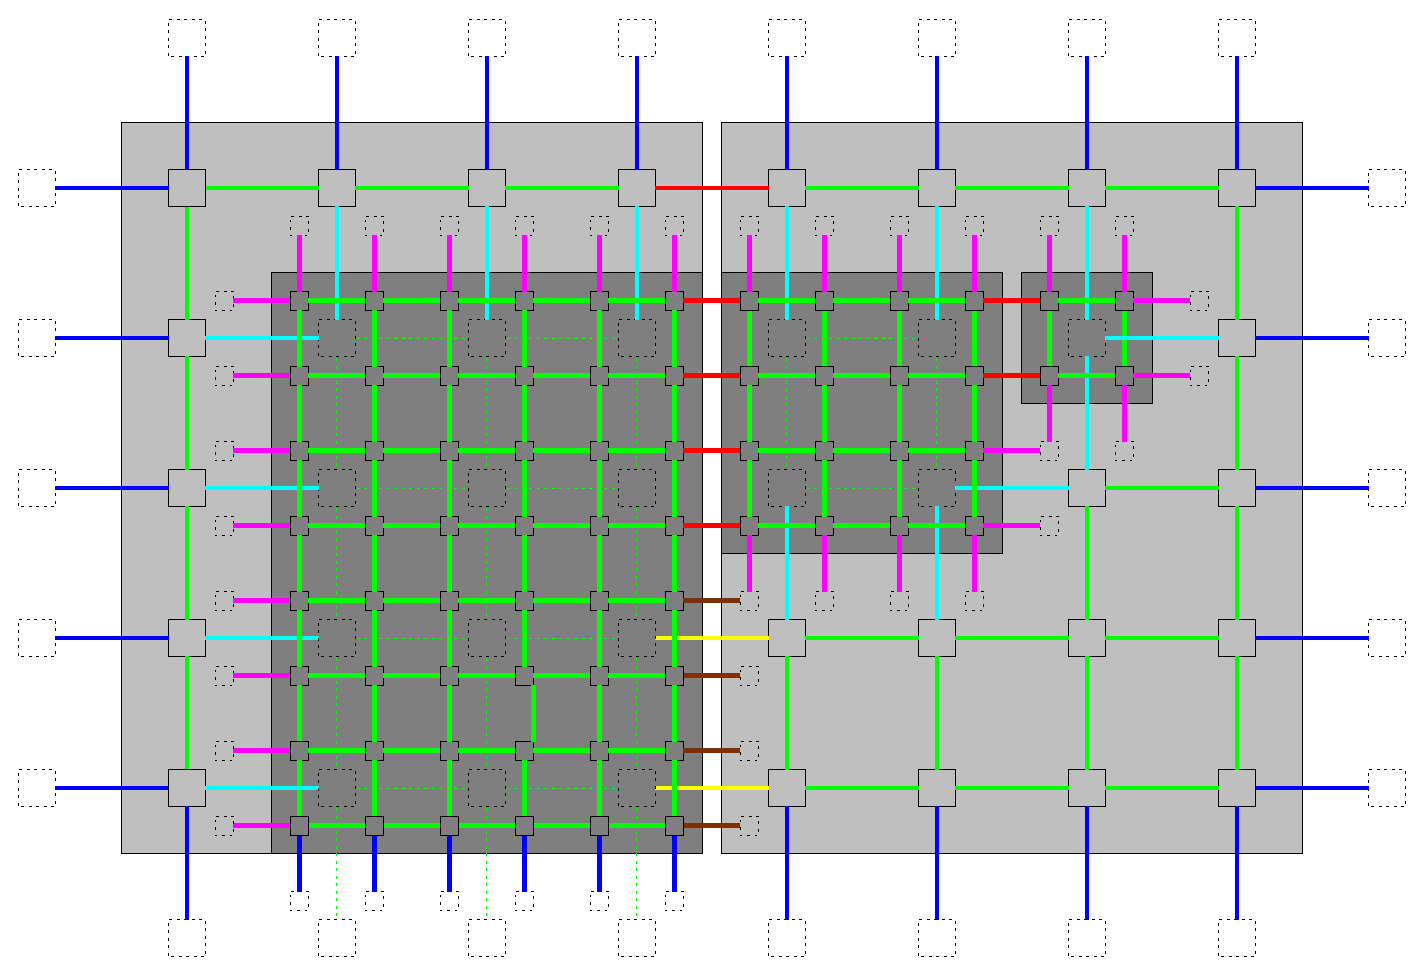
\epsfig{file=discret-step-1.eps,angle=90,width=1.75in}
\end{minipage} \
\begin{minipage}{2.25in}
\footnotesize
\raggedright
\begin{itemize}
  \item Significant additional complexity in setting up the linear system
  \item Internal stencils, neighbors, overlapped grids handled directly by \hypre
  \item Coarse-to-fine and fine-to-coarse connections handled zone-by-zone
\end{itemize}
% \begin{tabular}{ll}
% \textcolor{green}{internal} & Grid \\
% \textcolor{green}{overlapped internal} & Grid \\
% \textcolor{red}{neighbor} & Grid pair \\
% \textcolor{blue}{boundary} & Zone\\
% \textcolor{magenta}{fine-coarse parent} & Zone\\
% \textcolor{cyan}{coarse-fine child} & Zone\\
% \textcolor{brown}{fine-coarse parent--neighbor} & Zone\\
% \textcolor{yellow}{coarse-fine neighbor--child} & Zone\\
% \end{tabular}
\end{minipage}
\end{slide}

%=======================================================================
\begin{slide}{\large AMR RT Plan: Step 1a\\
              \normalsize  discretization}
\footnotesize
\begin{center}
\begin{minipage}{1.0in}
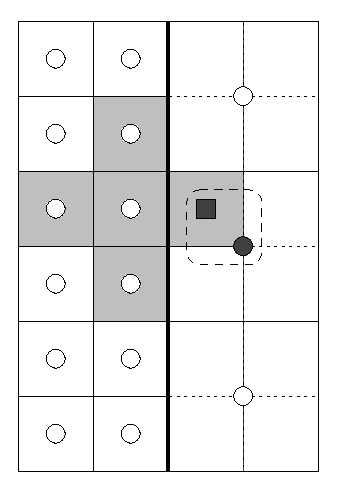
\epsfig{file=stencil0.eps,width=1.0in}
\end{minipage} \ \ 
\begin{minipage}{1.0in}
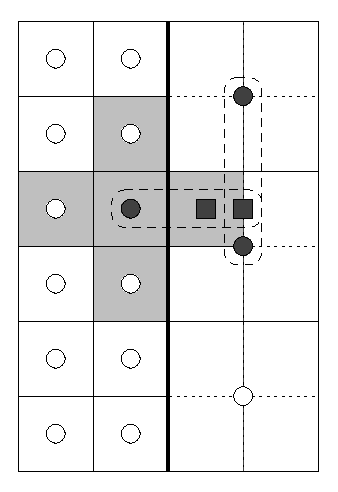
\epsfig{file=stencil1.eps,width=1.0in}
\end{minipage} \ \ 
\begin{minipage}{1.0in}
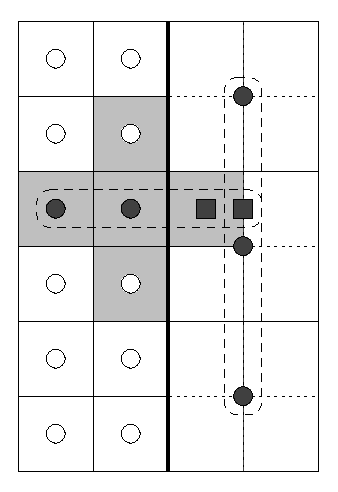
\epsfig{file=stencil2.eps,width=1.0in}
\end{minipage}
\begin{minipage}{4.0in}
\ \\
\begin{itemize}
\item Tradeoffs between accuracy and performance
\item Issues with nonsymmetric discretization?
\end{itemize}
\end{minipage}


\end{center}
\end{slide}

%=======================================================================
\begin{slide}{\large AMR RT Plan: Step 1b\\
              \normalsize  linear solve}
\small

\begin{itemize}
\item Wish to examine solver/preconditioner behavior:
\begin{itemize}
\item effect of problem anisotropies/discontinuities
\item effect of grid hierarchy characteristics
\item parallel performance and scalability
\end{itemize}
\item Suggestions for solvers to concentrate on?
\end{itemize}
\end{slide}

%=======================================================================
\begin{slide}{\large AMR RT Plan: Steps 2-3\\
              \normalsize  time-stepping and AMR RT testing}
\small
\begin{enumerate}
\item[2.] Hierarchical time-stepping issues
\begin{itemize}
\item solve only on coarser levels?
\item solve on coarser-level timesteps?
\item reuse previous solution as initial guess?
\end{itemize}
\item[3.] AMR RT test problems
\begin{itemize}
\item run unigrid tests with AMR turned on
\item additional AMR-specific tests
\end{itemize}
\end{enumerate}
\centerline{$\diamond$}
\end{slide}

\end{document}
